% !TEX root = ../main.tex
% !TeX spellcheck = en-US
\chapter{The BGK Equation}
\label{cha:BGK}
The Knudsen number \cref{knudsen} introduced by Danish physicist Martin Knudsen is a measure for the rarefaction of gases. In \cref{knudsen} $\lambda$ represents the mean free path and L the characteristic length \cite{Bernard} of a particle. The mean free path  describes the average distance a particle may travel between successive impacts [\textbf{WIKI}]. For idealized gases the mean free path can be calculated via \cref{lambda}. In \cref{lambda} $k_b$ is the Boltzman constant, p is the total pressure, T is the thermodynamic temperature and d is the hard shell diameter [\textbf{WIKI}]. 
\begin{multicols}{2}
	\begin{equation}
		Kn = \frac{\lambda}{L}
		\label{knudsen}
	\end{equation}
	\begin{equation}
		\lambda = \frac{k_bT}{\sqrt{2}\pi d^2p}
		\label{lambda}
	\end{equation}
\end{multicols}\noindent
For Kndusen numbers $Kn > 10^{-2}$ collisions are predominant in comparison to free transport, whereas for $Kn < 10^{-2}$ free transport becomes the predominant behavior compared to collision\cite{Bernard}. This difference in turn characterizes flows where the Bolzmann equation (collisions) or the Navier-Stokes equations (free transport) are valid. Hence the former \cref{Boltzmann} describes the dynamics of a gas flow, where f is the probability density distribution function for a particle at point $\textbf{x} \in \mathbb{R}^3$ with velocity $\xi \in \mathbb{R}^3$ at time $t \in \mathbb{R}$. 
\begin{equation}
	\partial_t f(\textbf{x}, \xi, t) + \xi \Delta_x f(\textbf{x},\xi,t) = Q(f,f)
	\label{Boltzmann}
\end{equation}
Originally Q is often the binary Boltzmann collision term, which can be intractable in pratice \cite{BGK}. Thus the BGK equation utilizes the BGK-Operator for the collision term Q(f,f) \cref{Collision}\cite{Bernard}.
\begin{align}
Q(f,f) &= \frac{M_f(\textbf{x},\xi,t) - f(\textbf{x},\xi,t)}{\tau(\textbf{x},t)} \label{Collision}\\
M_f(\textbf{x},\xi,t) &= \frac{\rho(\textbf{x},t)}{(2\pi T(\textbf{x},t))^{\frac{3}{2}}}\exp(-\frac{||\xi -U(\textbf{x},t)||^2}{2T(\textbf{x},t)})  \label{Maxwellian}\\
\tau(\textbf{x,t}) &= \frac{Kn}{\rho(\textbf{x},t)T^{1-\nu}(\textbf{x},t)} \label{Relaxation}
\end{align}
For many kinetic gas problems it is sufficient to replace the complexity of the Boltzmann collision term by a mean-free-path approach. $\tau$ is referred to as the relaxation time, considering the fact, that collisions tend to relax the distribution function to an equilibrium state $f_0$, where $f_0 = M_f$ the equilibrium state is approximated by a Maxwellian distribution function\cite{BGK}. In \cref{Maxwellian} $U(\textbf{x},t) = (u(\textbf{x},t),v(\textbf{x},t),w(\textbf{x},t))^T$ is the macroscopic velovity, $T(\textbf{x},t) \in \mathbb{R}$ and $\rho(\textbf{x},t)\in \mathbb{R}$is the temperature and density of the gas respectively. In \cref{Relaxation} $\nu\in\mathbb{R}$ is the exponent of the viscosity law of the gas. As a result one obtains th BGK equation which can be utilized for both hydrodynamic and rarefied regimes and meets global conservation as discussed in \cref{FeaturesSOD}. By multiplying the BGK equation with the collision invariants $\Phi(v) = (1,\xi,\frac{1}{2}\xi^2)^T$ and integrating over velocity space $d\xi$, one obtains the corrsponsing moments, \cref{moment1} to \cref{moment3}.
\begin{multicols}{3}
	\begin{equation}
		\rho(x,t) = \int f d\xi \label{moment1}
	\end{equation}
	\begin{equation}
		\rho u(x,t) = \int \xi f d\xi \label{moment2}
	\end{equation}
	\begin{equation}
		E(x,t) = \int \frac{1}{2}\xi^2 f d\xi \label{moment3}
	\end{equation}
\end{multicols}
\subsection{Macroscopic features of Hydrodynamic and Rarefied Gas Flows in the SOD-Shock Tube} \label{FeaturesSOD}
\begin{figure}[!htbp]
	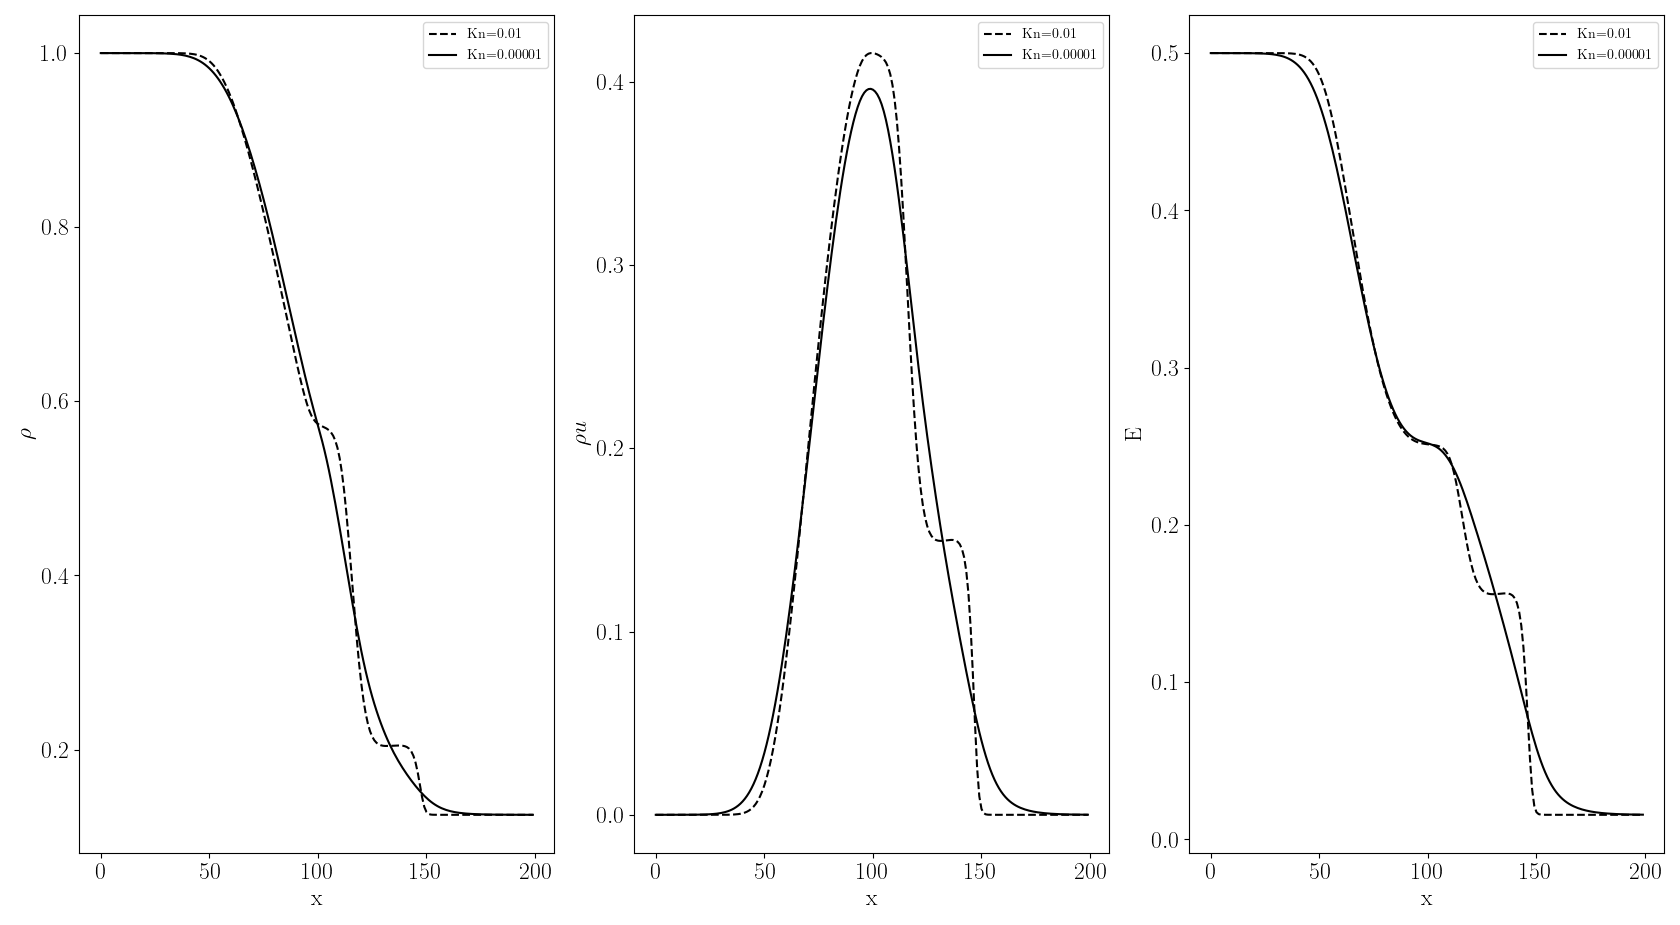
\includegraphics[width=\textwidth]{Macroscopic_Quantities_Original.png}
\end{figure}
- intrinsic code variables for hydro an rare add pls